\chapter{Marco Teórico}\label{ch:Marco Teórico}
En este capitulo...


\section{Origen e Historia}
Uno de los problemas del que se ocuparon los matemáticos del siglo XVIII es el que se conoce con el nombre del ``problema de la cuerda vibrante''. Este problema fue estudiado por d'Alembert y Euler (usando el método de propagación de las ondas) y un poco más tarde, concretamente en 1753, por Daniel Bernoulli. La solución dada por este difería de la proporcionada por los anteriores y consistió básicamente en expresar la solución del problema como superposición (en general infinita) de ondas sencillas. 

Las ideas de Bernoulli fueron aplicadas y perfeccionadas por Fourier, en 1807, en el estudio de problemas relacionados con la conducción del calor. Quedaron plasmadas por escrito en el libro clásico \emph{Théorie analytique de la chaleur}, publicado en 1822. Los razonamientos realizados por Fourier en este libro plantearon de manera inmediata numerosas controversias y cuestiones que han tenido una influencia significativa en la historia de la Matemática.


\subsection{El problema de la cuerda oscilante}

Uno de los problemas más interesantes que abordaron los científicos del siglo XVIII, y que aparece con frecuencia en problemas físicos relacionados con procesos oscilatorios, es el conocido como "El problema de la cuerda vibrante". Este se puede describir en su forma más elemental de la siguiente manera: Supongamos que tenemos una cuerda flexible y tensa, cuyos extremos están fijos, convenientemente, en los puntos $(0, 0)$ y $(\pi, 0)$ sobre el eje horizontal. Si la cuerda se tira de modo que su forma inicial corresponde a la curva definida por $y = f(x)$, y luego se suelta, la pregunta es: ¿Cuál será el movimiento resultante de la cuerda?

Los desplazamientos de la cuerda siempre se encuentran en un mismo plano, y el vector desplazamiento es perpendicular en cualquier momento. Para describir este movimiento se utiliza una función $u(x, t)$, donde $u(x, t)$ representa el desplazamiento vertical de la cuerda en la posición $x$ (con $0 \leq x \leq \pi$) y en el instante $t$ (con $t \geq 0$). El problema es determinar $u(x, t)$ a partir de $f(x)$.

El primer matemático que propuso un modelo adecuado para este problema fue Jean Le Rond d'Alembert. Bajo diversas hipótesis (asumiendo, por ejemplo, que las vibraciones son "pequeñas"), d'Alembert demostró en 1747 (\textit{Hist. de l'Acad. de Berlin, 3, 1747, pp. 214-219}) que la función $u(x,t)$ debe satisfacer las siguientes condiciones:

\begin{equation} \label{eq1}
	\begin{split}
		\frac{\partial^2 u(x,t)}{\partial t^2} &= \frac{\partial^2 u(x,t)}{\partial x^2}, \quad 0 < x < \pi, \ t > 0 \\
		u(x,0) &= f(x), \quad 0 \leq x \leq \pi \\
		\frac{\partial u(x,0)}{\partial t} &= 0, \quad 0 \leq x \leq \pi \\
		u(0,t) &= u(\pi,t) = 0, \quad t \geq 0.
	\end{split}
\end{equation}


La primera de estas condiciones es una ecuación en derivadas parciales de segundo orden, conocida como la \textit{Ecuación de Ondas}. La segunda ecuación establece la posición inicial de la cuerda, mientras que la tercera indica que la velocidad inicial de la cuerda es cero (recordando que, una vez desplazada a la posición $f(x)$, la cuerda es liberada). La última condición expresa que, para cualquier tiempo, los extremos de la cuerda permanecen fijos. En la figura \ref{fig:cuerda-vibrante} La variable $u = u(x,t)$ mide el desplazamiento sobre la vertical a tiempo $t > 0$ en la posición $x \in [0,\pi]$.

\begin{figure}[h]
	\centering
	
	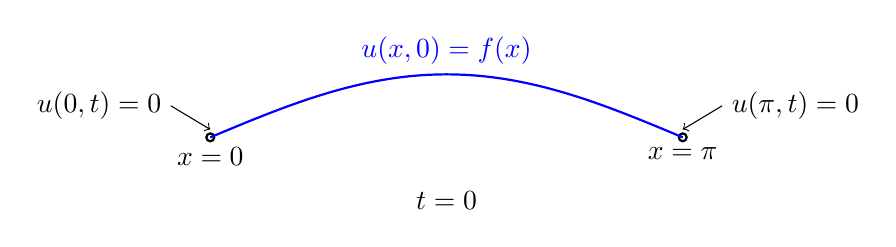
\begin{tikzpicture}[scale=1.0]
		% Ejes coordenados
		%\draw[->,ultra thick] (-0.5,0) -- (7,0) node[right] {$x$};
		%\draw[->,ultra thick] (0,-1) -- (0,2) node[above] {$u(x,t)$};
		
		% Extremos fijos en x=0 y x=L
		\draw[thick] (0,0) circle (0.05) node[below] {$x=0$};
		\draw[thick] (6,0) circle (0.05) node[below] {$x=\pi$};
		
		% Desplazamiento inicial de la cuerda
		\draw[domain=0:6,smooth,variable=\x,blue,thick] plot ({\x},{0.8*sin(180*\x/6)});
		
		% Etiqueta de la cuerda
		\node[above,blue] at (3,0.8) {$u(x,0) = f(x)$};
		
		% Condiciones de contorno (Movidas hacia arriba para evitar superposición)
		\draw[<-] (0,0.1) -- (-0.5,0.4) node[left] {$u(0,t)=0$};
		\draw[<-] (6,0.1) -- (6.5,0.4) node[right] {$u(\pi,t)=0$};
		
		% Indicación de tiempo inicial
		\node at (3,-0.8) {$t = 0$};
		
		% Flecha de tiempo (opcional)
		% \draw[->] (6.5,1) -- (6.5,1.5) node[right] {$t$ aumenta};
	\end{tikzpicture}
	\caption{Ilustración del problema de la cuerda vibrante.} 
	\label{fig:cuerda-vibrante}  % Etiqueta para la figura
\end{figure}
